The management structure can between companies based on their size and distribution. A company can have only one manager that tackles all the strategies from financial and to technical or it can have a hierarchy. 
The most generic hierarchy is described in \cref{subsec:levels}.
\subsection{Management levels}
\label{subsec:levels}
A generic hierarchy schema is usually based on 4 levels as in \cref{fig:levels}. The usual responsibilities for this levels are:

\begin{description}
\item[Top Management] is in charge of the strategies of the company.
\item[Branch/Senior Management] has the same responsibilities as the \textit{Top Management} but at a regional level in case the company is distributed in multiple locations.
\item[Middle Management] is in charge with organizing the people on competency levels (project managers, product managers, human resources managers)
\item[Execution] is not a a management level, it actually represents the persons who are doing the work for delivering the products of the company. In IT it is represented by: developers, quality engineers, recruiters.
\end{description} 

\begin{figure}[h]
\centering
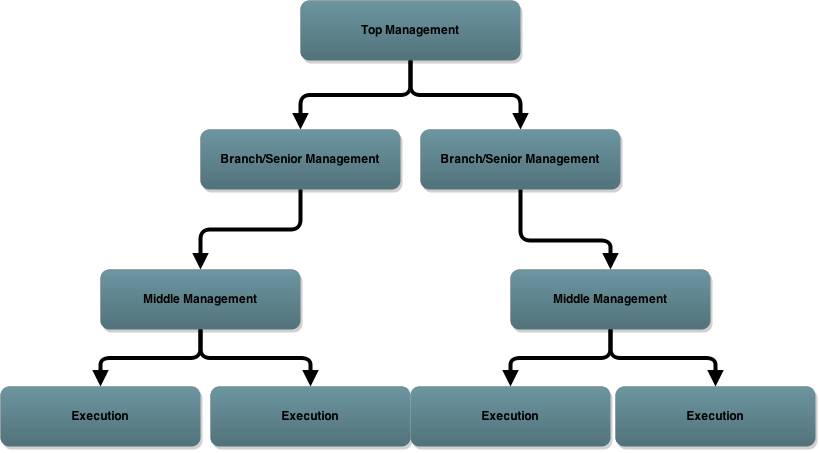
\includegraphics[width=0.8\textwidth]{img/levels.png}
\caption{Management Levels}
\label{fig:levels}
\end{figure}
Depending on the size of the company, the \textit{Senior Managers} may not exits, their tasks being handled by top management.
While in most cases the people managers are considered to be part of middle management, in my opinion they should not be considered part of the company hierarchy and should be considered a separate entity. If they are considered middle management, then it would be a contradiction for a senior manager to be a direct report of a middle manager, while the middle manager would be a direct report of a senior manager. People Management should be done in a matrix organization, because event senior managers need to be evaluated and motivated. In an organization based on hierarchy, the senior managers would be evaluated by top management based only on the performance of the company, but not on the degree of obtaining it's personal objectives.


\subsection{Management abilities}
A manager is not only a person in charge of filling out reports and proposing salary increases. A people manager is also in charge with addressing the different issues an employee has. In order to do this he must have a set of skills and continue to improve the quality and add value to the company. The kind of abilities are separated into three categories: technical, personal and interpersonal. The fact that a people manager should have technical skills rules in favour of \cref{subsec:techout} and \cref{subsec:techin} and is a strong indicator against \cref{subsec:hrdep}.

Some of the technical abilities are:
\begin{itemize}
\item Problem solving
\item Planning
\item Goal setting
\item Defining strategy
\item Time management
\end{itemize}

Problem solving and planning are needed in both helping and evaluating the performance of an employee, while time management and goal setting are useful in setting the development objectives.

The personal abilities are:
\begin{itemize}
\item Stress management
\item Integrity
\item Personal development
\end{itemize}

In crisis situation a people manager should be able to keep it's calm and guide his reports in solving the problems and also he a people manager has to be aware that his position does not mean that he knows everything there is. A people manager (everybody actually) should be continually improve his skills. In my case, the most important skills that I realized I did not quite master were coaching and evaluating \textbf{WHY} a person does the opposite of what it was expected.

The interpersonal skills are:
\begin{itemize}
\item Team development
\item Conflict management 
\item Coaching
\item Delivering feedback
\end{itemize}

The responsibilities of a people manager is to bring the best from his employees, but this does not mean to verify and just ask for things from them. When an employee is given new responsibilities, he may have the best intentions but he may not know the correct way to tackle them, in this situations the manager should begin a coaching period and help the person in cause develop their abilities.

Being in charge of both evaluating and motivating employees, people managers should be prepared to correct actions of employees and in order to do this, he should threat the causes of the actions and not the effects. As Simon Sinek describes in \cite{why} for finding out what is different from our expectations, the people manager should \textbf{Start with why}.
\subsection{Management relationships}
\label{subsec:relationships}
As long as a manager expects performance from his employees, both the employees and superiors expect performance from the manager. Although performance is expected from everyone, performance is differently understood by different members. Technical persons tend to understand performance as delivering bullet proof solutions while taking the as much time as needed. On the other hand managers see performance by the 80-20 rule, meaning that getting 80\% of the possible results using only 20\% of the needed time. Being in the middle between the execution level and the middle management, the people manager has to set and maintain the correct expectations on both sides.

\subsubsection{People Manager - Direct Report}
\label{sub-subsec:pmdr}
\todo{You with your people} \newline
The relationship between the 
\subsubsection{People Manager - Upper Management}
\label{sub-subsec:pmum}
\todo{You with your bosses} \newline

